\chapter{Design di app mobili}
\begin{redbar}
La \textbf{progettazione di applicazioni mobili} presenta una serie di sfide specifiche dovute alle caratteristiche dell'utente tipo e del contesto d'uso di questi dispositivi. Gli utenti di dispositivi mobili si trovano spesso in movimento, eseguono compiti nei brevi ritagli di tempo disponibili e, per questa ragione, non possono dedicare la loro attenzione in modo continuativo e concentrato come farebbero con un computer desktop. 
\end{redbar}

L’interazione con un’app mobile è spesso interrotta da eventi esterni, come notifiche, chiamate o situazioni ambientali che richiedono attenzione. Inoltre, gli utenti possono trovarsi in situazioni in cui non devono disturbare altre persone, come in luoghi pubblici o al cinema.

La progettazione mobile deve tenere conto di un’attenzione frammentata. L’utente potrebbe trovarsi in situazioni in cui altre attività, come guidare, richiedono la sua attenzione visiva, uditiva o l’uso delle mani, limitando le capacità di interazione con il dispositivo. Anche le condizioni ambientali, come l'illuminazione variabile o i rumori di fondo, possono influenzare l'uso dell'app e rendere più difficile per l'utente concentrarsi sul dispositivo. Di conseguenza, le applicazioni mobili devono essere progettate per minimizzare la complessità visiva e rendere l'interazione rapida e intuitiva.

Un’applicazione mobile si differenzia notevolmente da quelle per desktop, e adattare un'app desktop a un dispositivo mobile richiede scelte specifiche di progettazione. I limiti principali derivano dalle dimensioni dello schermo, dalla memoria disponibile e dalla modalità di interazione utente-dispositivo.
\begin{enumerate}
    \item \textit{Schermo dello smartphone:} Le dimensioni ridotte degli schermi mobili, tipicamente tra i 5 e i 7 pollici, offrono alta risoluzione ma limitano lo spazio disponibile. Questa caratteristica implica che l’interfaccia non può essere sovraccarica di elementi: solo le informazioni essenziali devono essere visualizzate, garantendo leggibilità e usabilità senza affollamento visivo.
    \item \textit{Memoria limitata:} Le risorse di memoria nei dispositivi mobili sono spesso inferiori rispetto ai computer desktop. Pertanto, è importante ridurre al minimo la dimensione dei file e dei dati processati dall’app, eliminando memory leaks e usando formati efficienti per il salvataggio delle informazioni.
\end{enumerate}
Un’altra importante differenza con i sistemi desktop è l’assenza di finestre multiple. In un dispositivo mobile, l’utente accede alle schermate sequenzialmente, e ogni schermata occupa l'intero spazio visibile. Questo limita il multitasking e obbliga a organizzare i contenuti in una sequenza logica e continua. Per applicazioni che, in ambiente desktop, richiedono più finestre aperte contemporaneamente, è necessario riorganizzare le funzioni in una serie di schermate sequenziali o, se possibile, concentrarsi solo su alcune funzionalità essenziali.

Diversamente dai computer desktop, i dispositivi mobili non supportano il multitasking per le app di terze parti. Quando l'utente riceve una chiamata, l'app in uso viene sospesa, richiedendo una progettazione che preveda la possibilità di interrompere l'applicazione senza perdere dati o stato. Quando l'utente riprende l’applicazione, questa dovrebbe essere in grado di riavviarsi rapidamente esattamente dallo stato precedente. Inoltre, se l'app necessita di modifiche nelle impostazioni del sistema, queste possono interrompere l’esperienza d’uso, e quindi si preferisce che il maggior numero possibile di configurazioni sia gestibile all’interno dell'app stessa.

Gli utenti mobili hanno generalmente poco tempo e non sono propensi a leggere istruzioni o sezioni di help approfondite. Per questo motivo, l’interfaccia deve essere intuitiva e basata su controlli standard facilmente riconoscibili. La navigazione dovrebbe essere strutturata con sequenze logiche di schermate che siano immediatamente comprensibili. Inoltre, è fondamentale includere un pulsante “back” in ogni schermata, che permetta all'utente di tornare indietro facilmente senza confusione.

\section{Stili di app mobili}
Le applicazioni mobili si differenziano tra loro non solo per lo scopo, ma anche per lo stile di interazione e la struttura delle informazioni. Ogni tipologia risponde a esigenze specifiche e offre un'esperienza utente diversa, che influenza l’interfaccia e l’organizzazione dei contenuti. Gli stili principali di applicazioni mobili includono: productivity app, utility app e immersive app. Ogni categoria si adatta a differenti esigenze e situazioni d’uso.

\subsection{Productivity application}
Le \textit{productivity app} sono pensate per supportare compiti che richiedono organizzazione e gestione di informazioni dettagliate. Applicazioni come la posta elettronica sono esempi tipici, poiché permettono di svolgere compiti importanti e richiedono un’interazione frequente. La user experience di queste applicazioni è focalizzata sul compito e sulle informazioni necessarie per completarlo, con un’interazione costante e dettagliata.

Un esempio classico di productivity app è Google Photo, che organizza e gestisce foto e video. La struttura dei dati in queste applicazioni è spesso organizzata in modo gerarchico, permettendo agli utenti di navigare tra diversi livelli di dettaglio e di eseguire operazioni specifiche a seconda del livello selezionato. L’interfaccia di queste applicazioni è semplice e pulita, con una schermata dedicata per ogni livello gerarchico, e l’utilizzo di controlli standard, che gli utenti riconoscono facilmente.

Generalmente, in questo tipo di applicazioni, l'utente può innanzitutto organizzare una lista di elementi, aggiungendo o rimuovendo voci a seconda delle necessità. A questo punto, è possibile navigare a livelli di dettaglio successivi: ogni livello presenta informazioni più specifiche sull'elemento selezionato, permettendo all’utente di compiere azioni mirate o approfondimenti direttamente su quel livello.

Le productivity app pongono l’enfasi sulle informazioni e sul compito, lasciando in secondo piano l’ambiente grafico o la ricchezza dell’esperienza visiva. Di solito, gli utenti possono impostare preferenze per ridurre scelte ripetitive e per focalizzarsi solo sulle operazioni essenziali, ottimizzando così il tempo e l’attenzione dedicata al task.

\subsubsection{Modi delle productivity app}
\begin{wrapfigure}{r}{0.35\textwidth}
  \vspace{-0.5cm}
  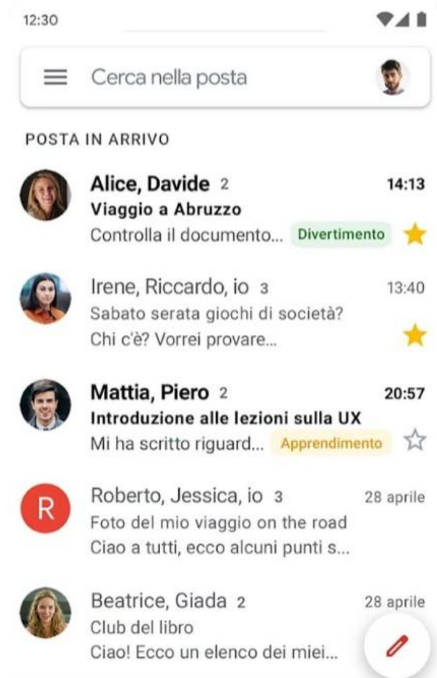
\includegraphics[width=0.35\textwidth]{images/esempio-gmail.PNG}
  \vspace{-1.2cm}
  %\caption{Birds}
\end{wrapfigure}

L’interfaccia di una productivity app presenta generalmente una lista di oggetti organizzata in una struttura ad albero, con una gerarchia che consente di scendere a livelli di dettaglio progressivi. Per esempio, un’app per la gestione della posta elettronica come Gmail mostra inizialmente una lista di conversazioni. Quando si seleziona una conversazione, viene visualizzata una nuova schermata che mostra i messaggi contenuti in quella conversazione, consentendo all’utente di navigare nei vari livelli dell’albero, partendo dalla radice e procedendo attraverso i nodi figli.

All'interno di queste app, gesti come lo swipe permettono di eseguire azioni rapide sulla conversazione stessa, come archiviare o segnare come letto/non letto, senza aprire nuove schermate. Per creare una nuova conversazione, basta toccare il pulsante con l’icona della matita, che apre una nuova schermata di composizione del messaggio.

Un principio chiave delle productivity app è l’utilizzo dell’approccio noun-verb, ossia “oggetto-azione.” Con questo metodo, l’utente sceglie prima l’oggetto e poi l’azione da compiere su di esso. Ad esempio, in un’app di posta elettronica, è possibile archiviare una conversazione eseguendo uno swipe o eliminarla con un semplice tap su un pulsante specifico. Questo approccio facilita la comprensione e la gestione delle azioni, in quanto l’animazione degli oggetti offre feedback immediato sull’avvenuta esecuzione, eliminando la necessità di alert o messaggi aggiuntivi.

L’approccio noun-verb è particolarmente vantaggioso per gli utenti mobili, poiché riduce gli errori di modo. Infatti, l’attenzione dell’utente è spesso frammentata e potrebbe non ricordare lo stato del sistema o il contesto in cui si trova, aumentando il rischio di errori. L’approccio noun-verb consente di svolgere le operazioni senza creare modi, ovvero situazioni in cui l’interpretazione delle azioni cambia in base allo stato del sistema.

La navigazione nelle productivity app è spesso arricchita da animazioni che facilitano l’esperienza utente. Quando si apre una nuova vista figlia, questa entra da destra e si sovrappone alla vista padre. Per tornare indietro, si può usare il pulsante "back" in alto a sinistra, che provoca uno scorrimento della vista figlia verso destra, rivelando di nuovo la vista padre. Questa struttura, simile a una pila, consente all’utente di mantenere un’idea chiara della gerarchia e della navigazione, con l’ultima schermata inserita che diventa la prima a uscire.

In alcuni casi, come nell’aggiunta di nuovi oggetti, l’interazione adotta l’approccio verb-noun, ovvero “azione-oggetto.” Un esempio è la composizione di un nuovo messaggio in un’app di posta elettronica: l’utente preme il pulsante “scrivi” (contrassegnato dall’icona di una matita) e accede a una nuova schermata, dove può iniziare a comporre il messaggio. Questa schermata viene visualizzata in modalità modale, salendo dal basso e coprendo la vista precedente per focalizzare l’attenzione dell’utente sulla composizione del messaggio.

Quando l’utente termina e invia il messaggio, la vista modale scorre verso il basso, rivelando di nuovo la schermata precedente e aggiungendo il nuovo elemento alla lista delle conversazioni con un’animazione, che funge da feedback visivo per confermare l’avvenuto invio.

Molte applicazioni per smartphone iniziano dalla radice dell’albero gerarchico, dove si trova la vista di default. Questa scelta, combinata con l’approccio noun-verb, rende l’applicazione rapida e facile da usare, con una riduzione degli errori. Iniziare dalla radice facilita l’accesso immediato alle funzioni principali e consente all’utente di orientarsi facilmente. Applicazioni come Gmail, WhatsApp, Telegram, Google Drive e BancoPosta utilizzano questo approccio per garantire semplicità e immediatezza.

\subsection{Utility application}
Le \textit{utility app}, o applicazioni di utilità, servono a compiere compiti semplici che richiedono un minimo intervento dell’utente. Il loro scopo principale è fornire informazioni essenziali su un argomento specifico, come nel caso delle applicazioni per le previsioni meteo. In queste app, non c’è struttura gerarchica: l’utente accede direttamente alle informazioni che gli interessano, e l’interazione è ridotta al minimo.

Per esempio, un’app meteo consente all’utente di visualizzare rapidamente le previsioni per varie città. L’interfaccia è tipicamente costituita da una o più liste non gerarchiche, facilitando così la lettura e l’accesso alle informazioni di interesse. Gli utenti possono modificare facilmente le impostazioni, come l’aggiunta di una nuova città o la visualizzazione delle temperature minime, direttamente dall’interno dell’applicazione, rendendo l’esperienza rapida ed efficace.

Nelle utility app, è comune che l’utente apporti frequenti modifiche alla configurazione, come nel caso delle app che monitorano stati o parametri in tempo reale. Queste applicazioni devono quindi essere progettate per semplificare le modifiche delle preferenze e per rispondere in modo dinamico ai cambiamenti dell’utente.

\subsection{Immersive application}
Le \textit{immersive app} sono applicazioni che forniscono un’esperienza immersiva, progettata per trattenere l’utente in un ambiente interattivo unico. Queste app, tipiche dei videogiochi o di esperienze virtuali, offrono ambienti ricchi di dettagli e occupano l’intero schermo del dispositivo, permettendo all'utente di esplorare e interagire con il contenuto in modo approfondito. L’attenzione dell’utente è catturata completamente, senza interruzioni o compiti collaterali.

Un esempio di immersive app è l’app IKEA Place, che permette agli utenti di visualizzare come i mobili si integrerebbero nello spazio domestico, utilizzando la realtà aumentata. L'interazione in queste applicazioni non segue i controlli standard, ma piuttosto introduce comandi unici e personalizzati. Parte dell’esperienza è data dalla scoperta dei comandi stessi e dal loro funzionamento, che coinvolge l’utente in un processo esplorativo.

Queste applicazioni spesso gestiscono grandi quantità di informazioni, ma le presentano in modo adatto al contesto, come dettagli grafici o elementi interattivi che potenziano l'esperienza visiva. L’utente si immerge nell’ambiente dell’app e interagisce con il contenuto come parte dell’esperienza stessa, invece di trattare semplicemente delle informazioni.

\section{Design patterns}
Il concetto di design pattern, o "modello di progettazione," fu introdotto inizialmente in architettura dall'architetto Christopher Alexander. 
\begin{center}
\textit{"Ogni modello descrive un problema che si ripresenta continuamente nel nostro ambiente e, successivamente, illustra il nucleo della soluzione a quel problema, in modo tale che questa soluzione possa essere utilizzata milioni di volte, senza mai applicarla nello stesso modo due volte."}
\end{center}
Questa idea fu poi estesa al design delle interfacce utente, con l’obiettivo di fornire soluzioni standardizzate per problemi comuni nel campo dell'interazione uomo-macchina (HCI).

I design patterns sono utili per risolvere problemi di progettazione ricorrenti e forniscono un linguaggio comune per i progettisti. Essi non sono né troppo generali né troppo specifici, il che permette di adattare la soluzione proposta alle particolarità del caso specifico. La loro funzione è quella di facilitare la comunicazione e il confronto tra designer: menzionare un design pattern riconosciuto offre immediatamente a tutti i partecipanti un'idea chiara di cosa si stia discutendo, permettendo di considerare direttamente eventuali alternative.

Ogni interfaccia utente è unica e progettata per rispondere a obiettivi e dati specifici. Tuttavia, ciò non significa che ogni interfaccia debba richiedere agli utenti di imparare nuove convenzioni per utilizzarla. I design patterns aiutano a creare un'interfaccia intuitiva, in cui gli utenti possono riconoscere rapidamente i comandi e le interazioni fondamentali, facilitando l’apprendimento e l’uso dell'applicazione.

Esempi di design patterns comuni nelle interfacce utente includono:
\begin{itemize}
    \item \textit{Accordion Menu:} un menu che si espande per rivelare le opzioni nascoste al suo interno, fornendo un’interazione intuitiva per navigare tra sezioni di contenuto correlate.
    \item \textit{Dropdown Menu:} una lista che si espande verso il basso quando selezionata, usata spesso per opzioni selezionabili che devono essere mantenute nascoste fino a quando non servono.
    \item \textit{Cards:} elementi a forma di "carta" che mostrano contenuti specifici e sono organizzati in griglie o pile, molto usati per contenuti visivi come foto e articoli.
    \item \textit{Breadcrumbs:} una rappresentazione della posizione corrente dell’utente all’interno della struttura dell’app, utile per facilitare la navigazione all’indietro.
    \item \textit{Hamburger Menu:} un’icona a tre linee parallele che, se selezionata, apre un menu nascosto con ulteriori opzioni di navigazione.
\end{itemize}
Nelle applicazioni mobili, soprattutto su Android, esistono design patterns specifici pensati per facilitare la navigazione e migliorare l’esperienza utente. Tra questi si trovano:
\begin{itemize}
    \item \textit{Toolbar e App Bar:} elementi fissi nella parte superiore dello schermo che includono opzioni come il menu e la barra di ricerca.
    \item \textit{Tabs:} consentono di navigare tra diverse sezioni di un’app all'interno della stessa schermata, mantenendo un contesto visivo chiaro.
    \item \textit{Navigation Drawer:} un menu laterale che si apre con uno swipe dal bordo dello schermo, rivelando opzioni di navigazione aggiuntive.
    \item \textit{Scrolling e Paging:} consentono di esplorare contenuti lunghi in modo fluido, con la possibilità di navigare tra pagine o sezioni con uno swipe.
\end{itemize}

\subsection{Dark patterns}
Oltre ai design patterns positivi, esistono anche i cosiddetti "dark patterns," termine coniato dal designer Harry Brignull nel 2010 per descrivere quegli schemi di progettazione che inducono deliberatamente gli utenti a prendere decisioni contrarie ai loro interessi. I dark patterns, che Brignull ha esposto in una galleria online e in una campagna di sensibilizzazione, mirano a manipolare gli utenti con tattiche come nascondere le opzioni di annullamento, rendere difficile la disiscrizione o spingere inconsapevolmente verso acquisti non desiderati.

Oggi, alcuni preferiscono sostituire il termine "dark pattern" con "deceptive design" o "design ingannevole" per evitare connotazioni negative legate al colore "dark". L’uso di questo tipo di progettazione è in calo, con un numero crescente di aziende e designer che riconoscono l’importanza di pratiche etiche e trasparenti nell’interazione uomo-macchina.

\subsection{Attention-capture damaging patterns}
L'economia dell'attenzione è un modello di business che si basa sul considerare l'attenzione degli utenti come una valuta. In pratica, le aziende tecnologiche progettano servizi digitali che catturano l'interesse degli utenti, utilizzando il tempo speso sulle piattaforme come una forma di pagamento. Questo modello è il motore dietro colossi tecnologici come Alphabet (Google) e Meta (Facebook, Instagram, WhatsApp), che traggono enormi profitti vendendo l'attenzione e, a volte, i dati degli utenti a inserzionisti.

Tuttavia, questo sistema ha conseguenze significative sul benessere digitale delle persone. Le piattaforme spesso impiegano tecniche che sfruttano le vulnerabilità psicologiche degli utenti, come la gratificazione immediata e il meccanismo delle ricompense variabili, per indurli a trascorrere sempre più tempo online. Il risultato è una perdita di controllo sugli obiettivi personali e una sensazione di pentimento per il tempo perso.

Un sottoinsieme di design pattern, noti come \textit{Attention-Capture Damaging Patterns (ACDPs)}, viene appositamente progettato per massimizzare l'uso continuo delle piattaforme digitali. Questi schemi spesso automatizzano processi per migliorare l'usabilità, ma lo fanno a scapito dell'autonomia decisionale degli utenti. Utilizzano strategie che includono:
\begin{itemize}
    \item \textit{Notifiche:} progettate per imitare segnali di pericolo, creando un senso di urgenza.
    \item \textit{Gratificazione immediata:} come i "like" o i commenti, che attivano il rilascio di dopamina nel cervello.
    \item \textit{Mescolanza di contenuti vecchi e nuovi:} una tattica mutuata dalle macchine da gioco, che mantiene gli utenti in uno stato costante di curiosità.
\end{itemize}
Alcuni esempi pratici di questi pattern includono:
\begin{enumerate}
    \item \textit{Raccomandazioni basate sui gusti dell'utente:} Le piattaforme suggeriscono contenuti che potrebbero piacere all'utente, ma con l'obiettivo di tenerlo impegnato più a lungo. Sebbene utili in alcune circostanze, queste raccomandazioni possono diventare una trappola, portando a un uso non intenzionale della piattaforma.
    \item \textit{Autoplay infinito:} Al termine di un video, un altro inizia automaticamente, impedendo agli utenti di fermarsi e riflettere. Questo meccanismo sfrutta la pigrizia decisionale e il principio della ricompensa variabile.
    \item \textit{Pull-to-refresh:} Simile al gesto di tirare la leva di una slot machine, scorrere verso il basso su uno smartphone ricarica la pagina e potrebbe rivelare nuovi contenuti, incentivando un comportamento compulsivo.
    \item \textit{Scrolling infinito:} Scorrendo verso l'alto su una pagina, nuovi contenuti vengono caricati automaticamente. Questo riduce l'attrito nella navigazione ma incoraggia sessioni di utilizzo senza fine.
\end{enumerate}

\section{Interfacce Android}
La progettazione delle interfacce per le applicazioni Android segue una serie di criteri fondamentali per migliorare l'esperienza utente. Questi principi si basano su una comprensione profonda delle capacità cognitive degli utenti, delle loro aspettative e dei modelli di interazione già conosciuti.

\subsection{Criteri}
Un design efficace utilizza gli elementi che gli utenti già conoscono. Questo principio si declina in tre aspetti fondamentali:
\begin{enumerate}
    \item \textit{Widget standard.} I widget sono gli elementi grafici predefiniti che gli utenti incontrano comunemente, come pulsanti, slider e menu a tendina. Utilizzare questi elementi riduce il tempo necessario per imparare a usare l'applicazione, poiché gli utenti riconoscono immediatamente le loro funzioni.
    \item \textit{Gesture standard.} Le gesture, come lo swipe o il pinch-to-zoom, sono comportamenti acquisiti nella navigazione digitale. Un'applicazione che adotta queste interazioni standard migliora l'accessibilità e la soddisfazione dell'utente.
    \item \textit{Metafore riconoscibili.} L'uso di metafore visive come un'icona del cestino per eliminare un file aiuta l'utente a comprendere rapidamente la funzione di un elemento. È importante scegliere immagini che siano culturalmente universali e intuitive.
\end{enumerate}
La \textit{discoverability} si riferisce alla capacità degli utenti di individuare facilmente le funzioni principali di un'interfaccia. Un errore comune è nascondere i controlli, rendendo l'interazione con l'applicazione più difficile.

Ad esempio, Material Design consiglia di evitare che i menu siano completamente nascosti dietro icone, se non necessario. Fornire un'indicazione visiva chiara aumenta la probabilità che l'utente esplori e utilizzi le funzionalità.

Una buona interfaccia deve rispondere rapidamente e chiaramente alle azioni dell'utente, rendendo l'interazione più naturale. Questo criterio comprende due aspetti principali:
\begin{enumerate}
    \item \textit{Manipolazione diretta.} Gli utenti dovrebbero essere in grado di interagire direttamente con gli elementi della schermata, come trascinare un oggetto o ridimensionarlo.
    \item \textit{Feedback immediato.} Ogni azione deve essere seguita da una reazione visibile. Ad esempio, quando si preme un pulsante, un cambiamento di colore o un'animazione può confermare che l'azione è stata registrata.
\end{enumerate}
L'interfaccia dovrebbe ridurre il carico cognitivo richiedendo agli utenti di selezionare, piuttosto che ricordare. Offrire menu a scelta o suggerimenti visivi facilita la navigazione e migliora l'efficienza.

Un esempio tipico è l'uso di menu a discesa per consentire la scelta di opzioni predefinite, invece di costringere l'utente a digitare manualmente.

Gli utenti devono sentirsi al comando durante l'interazione con un'app. Ciò si traduce in funzionalità come:
\begin{itemize}
    \item \textit{Orientamento chiaro.} Mostrare all'utente dove si trova nell'applicazione attraverso barre di navigazione o breadcrumbs.
    \item \textit{Navigazione inversa.} Funzioni come il pulsante "Indietro" permettono di annullare facilmente un'azione o tornare a una schermata precedente.
    \item \textit{Progress bar e undo.} Una barra di avanzamento fornisce un'indicazione chiara del progresso dell'utente, mentre l'opzione "Undo" offre un modo semplice per correggere errori.
\end{itemize}
Un'app efficace apprende e si adatta alle preferenze dell'utente.
\begin{itemize}
    \item \textit{Suggerimenti personalizzati.} L'applicazione può proporre impostazioni basate sull'uso passato.
    \item \textit{Personalizzazione attiva.} Offrire agli utenti la possibilità di modificare impostazioni come temi, layout o notifiche.
    \item \textit{Default sensati.} Impostazioni predefinite ben progettate riducono la necessità di personalizzazioni immediate.
\end{itemize}
Una buona interfaccia è coerente sia visivamente che comportamentalmente. Questo principio include:
\begin{itemize}
    \item \textit{Stesse gesture, stessa azione}. Un'azione deve sempre avere lo stesso risultato, indipendentemente dal contesto.
    \item \textit{Evitare i modi}. Un’interfaccia che cambia funzione di un elemento in base al contesto può confondere.
    \item \textit{Coerenza tra widget e funzioni}. Un widget, come un bottone o un campo di testo, deve sempre comportarsi in modo prevedibile.
    \item \textit{Temi uniformi}. L'aspetto grafico deve essere armonizzato per creare un'identità visiva forte.
\end{itemize}

\subsection{Material design}
Material Design è un linguaggio visivo sviluppato da Google per garantire un’esperienza coerente, intuitiva e moderna su tutte le piattaforme e i dispositivi Android.

Material Design si ispira alle proprietà fisiche dei materiali del mondo reale per creare un’interfaccia digitale che sembri tattile e naturale. Ogni elemento, come pulsanti e schede, simula comportamenti fisici, come la luce e le ombre, per fornire una percezione visiva di profondità e gerarchia.

\subsubsection{Lists}
Le liste sono un componente centrale del Material Design, utilizzate per organizzare informazioni in un formato verticale continuo e per mostrare contenuti multipli in modo ordinato. Possono includere testo e immagini, con l’obiettivo di aiutare gli utenti a trovare e agire su un elemento specifico. Le liste si classificano in tre dimensioni: a una linea, due linee o tre linee.

Le liste sono progettate per essere continue e coerenti, in modo che l'utente possa scorrere agevolmente senza interruzioni visive.

\subsubsection{Cards}
Le cards sono un altro elemento distintivo del Material Design.
Sono elementi versatili che rappresentano un contenuto organizzato intorno a un singolo argomento. Possono contenere testi, immagini, pulsanti e icone, offrendo un punto di accesso a dettagli più approfonditi o ulteriori navigazioni. La loro flessibilità permette l'uso in vari layout, come griglie, elenchi verticali o caroselli.

\subsubsection{Buttons}
I bottoni sono componenti essenziali che comunicano azioni disponibili. In Material Design, i bottoni hanno angoli completamente arrotondati e dimensioni tali da contenere comodamente il testo dell’etichetta. Possono includere icone opzionali, posizionate a sinistra rispetto al testo. È importante usarli con moderazione per evitare di compromettere la gerarchia visiva.

\subsubsection{Floating Action Buttons (FAB)}
Il Floating Action Button è progettato per evidenziare l'azione più importante in una schermata, come "Aggiungi", "Condividi" o "Avvia". Questo bottone fluttuante è persistente durante lo scorrimento e si trova solitamente in un contenitore arrotondato sopra la barra di navigazione.

\subsubsection{Alerts}
Gli avvisi sono messaggi generati dal sistema per informare l'utente di situazioni critiche o che richiedono una decisione immediata. Possono essere utilizzati per segnalare errori, chiedere conferme o fornire notifiche importanti.
Gli avvisi devono essere chiari, immediatamente riconoscibili e mai troppo invasivi.

\subsubsection{Bottom Sheets}
I bottom sheets sono pannelli che si sollevano dal bordo inferiore dello schermo, mostrando contenuti o azioni supplementari. Possono essere di due tipi: standard, utilizzati per integrare i contenuti principali (come un lettore audio), o modali, che offrono un’alternativa ai menu inline, spesso coprendo l’intero schermo.

Questo componente è particolarmente utile per mantenere l'interfaccia pulita, mostrando solo le opzioni rilevanti quando necessario.

\subsubsection{Side Sheets}
I side sheets mostrano contenuti secondari ancorati ai lati dello schermo. Sono utili per azioni come filtri o opzioni che influenzano i contenuti principali. Possono essere standard, ideali per schermi ampi, o modali, pensati per dispositivi con spazi più ristretti.

\subsubsection{Tabs}
Le tabs organizzano i contenuti in diverse categorie, offrendo un metodo di navigazione intuitivo tra sezioni correlate. Ogni tab include un'etichetta e, opzionalmente, un’icona. L’utente può passare da una tab all’altra scorrendo lateralmente o cliccando direttamente sull’etichetta.

\subsubsection{Barre dell’applicazione}
Material Design distingue tra due tipi di barre applicative: la top app bar e la bottom app bar.
\begin{itemize}
    \item La \textit{top app bar} include il titolo della schermata corrente e opzioni di navigazione come il menu "hamburger" o una freccia per tornare indietro. Scorrendo verso il basso, questa barra scompare per massimizzare lo spazio visibile.
    \item La \textit{bottom app bar}, invece, ospita fino a quattro pulsanti di azione e può integrare un Floating Action Button. È adatta a schermate con molte opzioni di azione.
\end{itemize}

\subsubsection{Navigation Bar}
La barra di navigazione (precedentemente chiamata "bottom navigation") consente l'accesso rapido a 3-5 destinazioni di pari importanza. Ogni destinazione è rappresentata da un’icona e, opzionalmente, un’etichetta. Questa barra è ideale per le app che richiedono un accesso costante a più sezioni principali, come "Home", "Profilo" e "Impostazioni".

\subsubsection{Transizioni}
Le transizioni definiscono il modo in cui i contenuti si spostano e interagiscono durante la navigazione. Possono essere:
\begin{itemize}
    \item Avanti e indietro, per navigare tra livelli gerarchici.
    \item Laterali, per esplorare contenuti paralleli, come il passaggio tra tabs.
\end{itemize}

\subsubsection{Sistema cromatico}
Material Design 3 (M3) introduce un sistema cromatico sofisticato per garantire coerenza, accessibilità e personalizzazione nelle interfacce utente. Questo sistema consente di creare temi statici partendo da un colore di riferimento, utilizzando algoritmi per generare palette cromatiche coerenti e ben bilanciate. Un aspetto interessante è la sua versatilità: i temi creati con M3 sono applicabili anche su piattaforme diverse da Android, come iOS.

Il sistema cromatico è centrale nella progettazione visiva:
\begin{itemize}
    \item Promuove una coerenza visiva che rafforza l'identità del brand.
    \item Integra principi di accessibilità, garantendo contrasti ottimali per diverse situazioni visive.
    \item Offre opzioni di personalizzazione per adattarsi a ogni esigenza di design.
\end{itemize}
Il modello cromatico di M3 si basa su tre componenti fondamentali:
\begin{enumerate}
    \item \textit{Ruoli dei colori (color roles):} Ogni elemento visivo è associato a un ruolo specifico, come "primary" per i pulsanti principali o "background" per lo sfondo generale.
    \item \textit{Assegnazione dinamica:} Gli elementi visivi ricevono un colore sulla base del loro ruolo.
    \item \textit{Algoritmo della palette:} A partire da un colore di riferimento, noto come seed color, il sistema genera tonalità e livelli di luminosità, adattandoli ai vari contesti.
\end{enumerate}
I ruoli non indicano un colore preciso, ma descrivono il loro utilizzo. Ad esempio, un pulsante etichettato come "primary" utilizzerà un colore specifico in base alla modalità chiara o scura selezionata.

Ecco alcuni ruoli comuni:
\begin{itemize}
    \item \textit{Primary:} Colore degli elementi interattivi principali.
    \item \textit{Secondary:} Accenti visivi e complementi.
    \item \textit{Tertiary:} Variazioni stilistiche opzionali.
    \item \textit{Background:} Colore dello sfondo generale.
    \item \textit{Surface:} Superfici come schede o finestre.
    \item \textit{Error:} Colore per messaggi di errore.
    \item \textit{Outline:} Bordature o contorni di elementi.
    \item \textit{On-Roles:} Testi o icone sovrapposti a uno sfondo, come "on-primary" o "on-background".
\end{itemize}
Material Design 3 utilizza un algoritmo avanzato noto come Material Color Utilities (MCU). Questo sistema:
\begin{enumerate}
    \item Richiede un seed color come input.
    \item Genera 5 colori complementari chiave (key colors).
    \item Crea una palette di tonalità per ciascun key color, con 13 livelli di luminosità.
    \item Assegna i colori generati ai ruoli principali dell'interfaccia.
\end{enumerate}
La distribuzione dei colori avviene in base a:
\begin{itemize}
    \item La modalità del tema (chiara o scura).
    \item Le regole di accessibilità, per garantire che ogni elemento sia ben visibile.
\end{itemize}
Material Design 3 semplifica il processo di creazione dei temi grazie a strumenti integrati, come il plug-in Material Theme Builder per Figma. Questo strumento consente di:
\begin{enumerate}
    \item Inserire un seed color.
    \item Generare automaticamente una palette cromatica.
    \item Assegnare i colori generati ai color roles.
    \item Applicare i temi a componenti predefiniti.
\end{enumerate}
Utilizzando il M3 Design Kit in Figma, si possono creare prototipi di interfaccia che rispettano i ruoli cromatici. Il processo tipico prevede:
\begin{enumerate}
    \item Selezione del colore rappresentativo del brand come seed.
    \item Generazione automatica della palette e aggiornamento del tema.
    \item Applicazione del tema ai componenti dell'interfaccia tramite la funzione "swap".
\end{enumerate}

\section{Interfacce IOS}
Progettare interfacce per iOS richiede il rispetto di criteri specifici che garantiscano un’esperienza utente fluida e coerente. Vedremo i principi fondamentali come l’autenticazione, la navigazione, il branding e altri elementi chiave che rendono un’app intuitiva e in linea con le aspettative degli utenti iOS.

\subsection{Criteri}
Un aspetto essenziale della progettazione di applicazioni è l’implementazione del \textit{processo di autenticazione}. Per migliorare l’esperienza utente, si consiglia di posticipare il più possibile il momento in cui l’utente deve effettuare il login, preferibilmente dopo aver dimostrato i vantaggi di tale operazione. Minimizzare i dati da inserire è altrettanto importante: l’utilizzo di metodi come l’accesso tramite social network o il riconoscimento biometrico può ridurre significativamente gli attriti.

L’\textit{inserimento di dati} manuali può essere un compito noioso e incline agli errori. È preferibile utilizzare selettori piuttosto che richiedere all’utente di digitare informazioni, ricorrendo a dati già presenti nel sistema (come contatti o indirizzi). Gli sviluppatori possono inoltre sfruttare impostazioni predefinite, validazioni dinamiche e suggerimenti visivi per semplificare l’esperienza.

Le \textit{gesture}, ovvero i gesti tattili, sono un elemento distintivo delle interfacce mobili. Le applicazioni iOS dovrebbero adottare gesture standardizzate, evitando di associare comportamenti non convenzionali a queste ultime. 

Le \textit{viste modali} sono strumenti utili per focalizzare l’attenzione dell’utente su compiti specifici. Queste viste possono occupare lo schermo parzialmente o completamente e includono sempre controlli chiari per completare o annullare l’operazione. È fondamentale che i compiti modali siano pochi, semplici e brevi.

Un’app ben progettata mantiene chiaro il percorso di \textit{navigazione} per l’utente. Questo obiettivo può essere raggiunto utilizzando componenti standard come barre di navigazione, barre delle tab e controlli di paginazione. Inoltre, l’adozione di gesture familiari, come il gesto di scorrimento per tornare indietro, rafforza ulteriormente l’intuitività dell’interfaccia.

Il \textit{branding} deve essere discreto e ben integrato nella grafica dell’app, evitando di risultare invasivo. Gli elementi visivi, come i loghi, dovrebbero essere coerenti in tutta l’app ma non collocati nella barra di navigazione, dove potrebbero distrarre l’utente.

La \textit{schermata di avvio} di un’applicazione iOS dovrebbe ripristinare il contesto dell’utente e permettere di riprendere eventuali attività interrotte. Questo approccio riduce la frustrazione e migliora la continuità dell’esperienza. La schermata di avvio deve essere identica all'interfaccia principale, senza contenere testi o elementi dipendenti dalla localizzazione, al fine di garantire coerenza e rapidità.

\subsection{Strumenti}
Le principali funzionalità offerte dal sistema operativo IOS sono Haptic Touch, le notifiche, i widget della schermata Home e Siri.
\begin{itemize}
    \item \textit{Haptic Touch.} Haptic Touch è una tecnologia che combina il gesto di una pressione prolungata sullo schermo con un feedback tattile, simulando la sensazione di premere un tasto fisico. Questa interazione può attivare un menu contestuale, mostrare contenuti aggiuntivi o fornire un'anteprima.

    Haptic Touch supporta diverse interazioni, come il "peek" e il "pop". La pressione iniziale, seguita da una vibrazione, consente di sbirciare un contenuto (peek) visualizzando una preview. Mentre una pressione prolungata pressione permette di accedervi completamente (pop). Se al peek segue uno swipe verso l'alto viene mostrato un menù di action buttons per l'item selezionato.

    \item \textit{Notifiche.} Le notifiche rappresentano uno strumento fondamentale per comunicare informazioni importanti all'utente. iOS supporta notifiche locali e push, che possono essere configurate per includere un titolo, un testo descrittivo e un suono. È interessante notare che le notifiche non mostrano il nome o il logo dell'app, concentrandosi esclusivamente sul contenuto rilevante.

    Le notifiche possono apparire sotto forma di banner, avvisi o direttamente sulla schermata di blocco. L'interazione con queste notifiche è altrettanto versatile: un semplice tap permette di aprirle, mentre uno swipe verso l'alto le cancella. Inoltre, con una pressione prolungata (Haptic Touch) o uno swipe verso il basso, l'utente può visualizzare una versione espansa che mostra maggiori dettagli o opzioni di azione.

    \item \textit{Home Screen Widgets.} I widget della schermata Home sono un modo pratico per offrire informazioni essenziali o funzionalità rapide direttamente sulla schermata principale o nella vista "Oggi". Ogni app può includere più widget, progettati per essere efficienti e consumare meno risorse grazie alla gestione intelligente della cache. I widget possono contenere bottoni, testo, immagini e altre componenti interattive.

    \item \textit{Siri.} L'integrazione con Siri permette alle applicazioni di iOS di offrire esperienze vocali naturali e intuitive. Utilizzando App Intents, gli sviluppatori possono definire i task supportati dall'app, convalidare gli input dell'utente, eseguire i compiti richiesti e fornire un feedback. Siri Shortcuts consente inoltre di semplificare le interazioni, proponendo opzioni chiare e immediate.
\end{itemize}

\subsection{Human Interface Guidelines}
La progettazione delle interfacce utente per applicazioni iOS è regolata da una serie di linee guida chiamate Human Interface Guidelines (HIG). Queste direttive hanno lo scopo di creare esperienze intuitive e coerenti per gli utenti, promuovendo pratiche che rendano le interazioni con le app fluide ed efficaci.
Vedremo alcuni degli elementi chiave utilizzati nelle interfacce grafiche, come barre, viste e controlli. Questi componenti non solo migliorano la navigazione e l'usabilità, ma offrono anche agli sviluppatori una base solida per costruire esperienze utente di alta qualità.

\subsubsection{Bar}
\begin{itemize}
    \item La status bar è un elemento essenziale dell'interfaccia iOS che fornisce informazioni sullo stato corrente del dispositivo, come la connessione di rete, l'orario e il livello della batteria. Questo componente viene generato automaticamente dal sistema operativo e dovrebbe essere sempre visibile. In caso di operazioni lunghe, come il caricamento di dati dalla rete, può essere utilizzato un indicatore di progresso indeterminato per comunicare all’utente che l’operazione è in corso.

    \item La navigation bar è fondamentale per la navigazione all'interno di un'applicazione. Essa include un pulsante "Indietro", un titolo che rappresenta la schermata corrente e, talvolta, un controllo segmentato o un pulsante aggiuntivo. Tuttavia, non è necessaria se la vista corrente non permette ulteriori navigazioni. iOS consente anche di utilizzare titoli grandi per migliorare la gerarchia visiva, rendendo più chiaro all'utente in quale sezione dell’app si trova.

    \item La toolbar contiene bottoni o etichette che permettono di eseguire azioni rilevanti nella vista corrente. Deve essere compatta e chiara, con un massimo di cinque icone selezionate da un set predefinito e prive di didascalie, oppure tre etichette di testo dinamiche.

    \item La tab bar è utilizzata per navigare tra diverse sezioni di un’app. Ogni tab può includere un'icona personalizzata e una breve etichetta. Sebbene sia possibile avere fino a cinque tab, in caso di sezioni aggiuntive viene mostrata una voce “Altro”. La tab bar è sempre visibile e può includere badge dinamici per indicare notifiche o aggiornamenti. 
    
    È importante utilizzare il numero minimo necessario di tab per facilitare la navigazione, mantenendoli visibili anche quando il loro contenuto non è disponibile. Per ogni tab, è consigliabile utilizzare termini sintetici ed evitare etichette generiche come "Home", che potrebbero risultare ambigue.

    \item Le sidebars offrono un metodo pratico per navigare in un’applicazione, fornendo accesso rapido alle principali aree o collezioni di contenuti. Gli utenti si aspettano di poter mostrare o nascondere la sidebar tramite il gesto integrato di swipe dal bordo dello schermo. Tuttavia, si consiglia di limitare la gerarchia a non più di due livelli, per evitare complessità. Nelle applicazioni iOS, è preferibile considerare l’uso di una tab bar al posto di una sidebar, poiché risulta più intuitiva e conforme alle linee guida di design.
\end{itemize}

\subsubsection{Views}
\begin{itemize}
    \item Una collezione rappresenta un insieme ordinato di contenuti disposti in un layout altamente visivo, che può essere una griglia o una fila orizzontale. Questo approccio è ideale per contenuti visivi come immagini, mentre per il testo è preferibile utilizzare una tabella. Gli utenti possono interagire tramite tap per selezionare un elemento, tenere premuto per modificare o effettuare uno swipe per scorrere.

    \item Le liste e le tabelle sono strutture utilizzate per presentare dati in colonne e righe, rendendo i contenuti facilmente leggibili e scansionabili.
    
    Le tabelle sono uno strumento versatile per mostrare contenuti organizzati. Sono strutturate in una singola colonna e possono essere scorrevoli verticalmente. Gli elementi nelle tabelle possono essere raggruppati in categorie (viste grouped) o elencati in modo semplice (viste plain). Queste tabelle devono essere aggiornate frequentemente per riflettere dati in tempo reale.

    Le righe delle tabelle possono variare in base al formato dei dati. Possono includere titoli, sottotitoli o valori correlati disposti su due colonne (value1 e value2), rendendo il contenuto facilmente leggibile e organizzato.

    \item I pulsanti sono progettati per attivare azioni immediate. È fondamentale che siano visivamente distinguibili dagli altri elementi dell'interfaccia.

    Ogni pulsante dovrebbe avere un'etichetta di testo, un'icona o una combinazione di entrambi. Lo spazio intorno al pulsante deve essere sufficiente per evidenziarlo visivamente. Si consiglia di limitare il numero di pulsanti visivamente prominenti a uno o due per schermata per evitare confusione.

    I Floating Action Buttons (FAB) sono widget fondamentali nell'ecosistema Android, ma non sono raccomandati per le applicazioni iOS. Gli utenti iOS potrebbero non comprendere come interagire con questo elemento, poiché non è parte delle loro convenzioni di utilizzo. Invece, è preferibile posizionare un pulsante per le azioni principali nella parte superiore destra della navigation bar, rendendo l'azione più intuitiva e coerente con le aspettative degli utenti.

    \item I segmented controls sono utili per presentare un numero limitato di opzioni strettamente correlate, che gli utenti possono confrontare rapidamente. Possono essere utilizzati per alternare viste o modalità all'interno della stessa schermata e possono contenere testo, icone o entrambi. Il numero ideale di opzioni è compreso tra 2 e 5. È consigliabile implementare animazioni fluide per evidenziare le modifiche di stato, fornendo un feedback immediato agli utenti.

    \item Gli alert sono notifiche asincrone utilizzate solo per comunicare informazioni critiche. Questi elementi interrompono l’attività corrente e richiedono all’utente di prendere una decisione. Gli alert devono essere progettati con titoli e testi brevi, con uno o più pulsanti per le azioni.

    Gli alerts sono viste modali progettate per fornire informazioni importanti e non attese che l’utente deve affrontare immediatamente. Sono ideali per segnalare problemi, avvisare dell’eliminazione di dati o confermare un acquisto. Non dovrebbero essere utilizzati per semplici comunicazioni informative o azioni comuni che possono essere annullate, anche quando queste sono distruttive.

    \item Gli action sheets vengono visualizzati su richiesta dell'utente per presentare opzioni relative all'azione corrente. Hanno un layout chiaro, senza contenuti scrollabili, e includono sempre un pulsante per annullare l'operazione.

    Gli action sheets rappresentano un’alternativa efficace agli alert o ai menu per offrire scelte relative a un’azione intenzionale da parte dell’utente. Un esempio comune è l’opzione per annullare la scrittura di un’email. L’action sheet deve includere un pulsante per annullare l’operazione, posizionato in fondo, oltre a opzioni aggiuntive correlate all’azione.

    \item Le activity views sono progettate per eseguire task specifici nel contesto corrente, come la condivisione di un documento o l’invio di un file. Questi elementi sono forniti di default ma possono essere personalizzati. Gli sviluppatori possono utilizzare pulsanti di azione per attivare queste viste, garantendo un’interazione semplice e diretta.
\end{itemize}

\subsubsection{Controls}
I controlli permettono agli utenti di interagire con l’applicazione, inserendo dati o selezionando opzioni. Un esempio importante sono i text fields, che devono supportare tastiere appropriate al tipo di input richiesto e funzioni come l’input predittivo per migliorare l’efficienza.
